\documentclass[11pt]{article}
\usepackage[margin=1in]{geometry}
\usepackage{graphicx}
\usepackage{amsmath}
\usepackage{amssymb}

\setlength\parindent{0pt}
\setlength{\parskip}{12pt}

\begin{document}

\begin{center}
\Large \textbf{CS4013/5013 Assignment 2}\\[0.5em]
\large Fall 2025\\[0.5em]
\normalsize Colby Frison | OUID: 113568816\\[1em]
\end{center}

\section*{Task 1: Hill Climbing Local Search Algorithm}

\subsection*{\textit{(1)} Figure 2: Error vs Search Round}

The following figure shows the convergence of the hill climbing local search algorithm. The x-axis represents the search round and the y-axis represents the error $er(w)$.

\begin{figure}[h!]
    \centering
    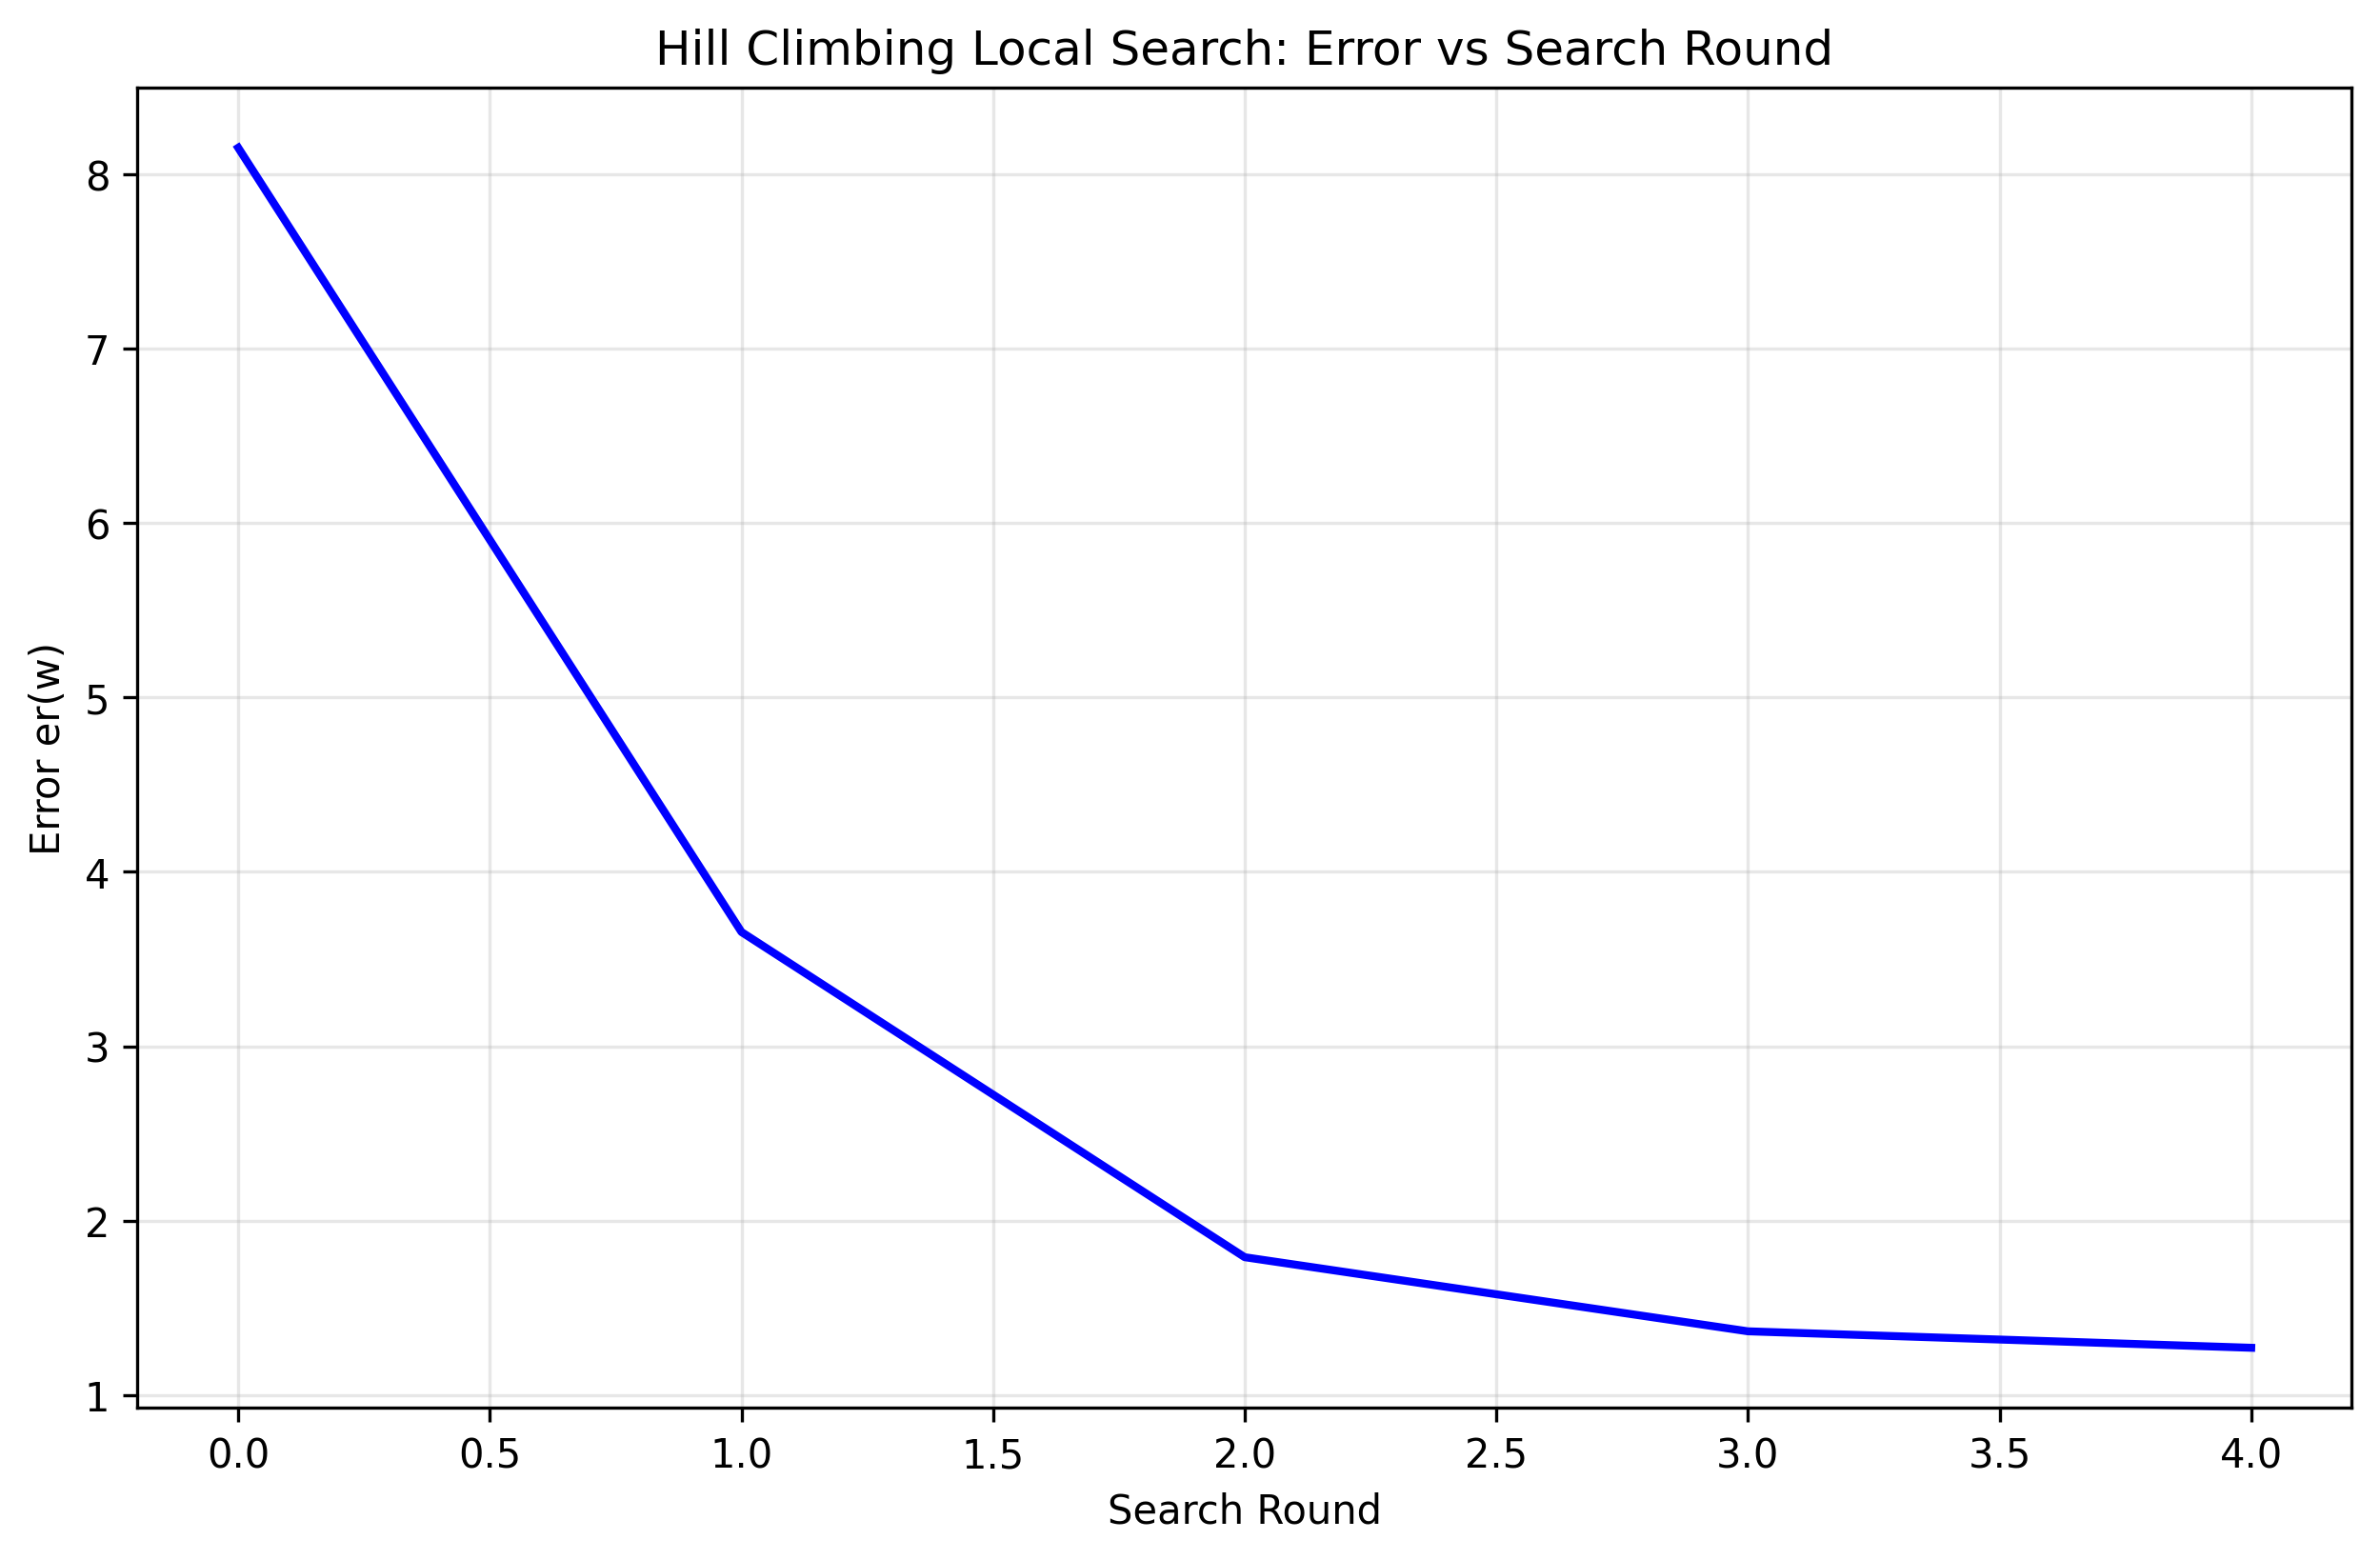
\includegraphics[width=0.75\linewidth]{../../local_search_error.png}
    \caption{Error $er(w)$ versus search round for hill climbing local search algorithm}
    \label{fig:local}
\end{figure}

\subsection*{\textit{(2)} Optimal Solution}

The optimal weight vector $w$ and corresponding error $er(w)$ returned by the hill climbing local search algorithm are:

\setcounter{equation}{2}
\begin{equation}
\label{eq:w_local}
w = [1, -1, 1, -1, 1, 1]
\end{equation}

\begin{equation}
\label{eq:er_local}
er(w) = 1.2713864306784661
\end{equation}

\newpage

\section*{Task 2: Genetic Algorithm}

\subsection*{\textit{(3)} Figure 3: Error vs Generation}

The following figure shows the convergence of the genetic algorithm across generations. The x-axis represents the generation number and the y-axis represents the error $er(w)$.

\begin{figure}[h!]
    \centering
    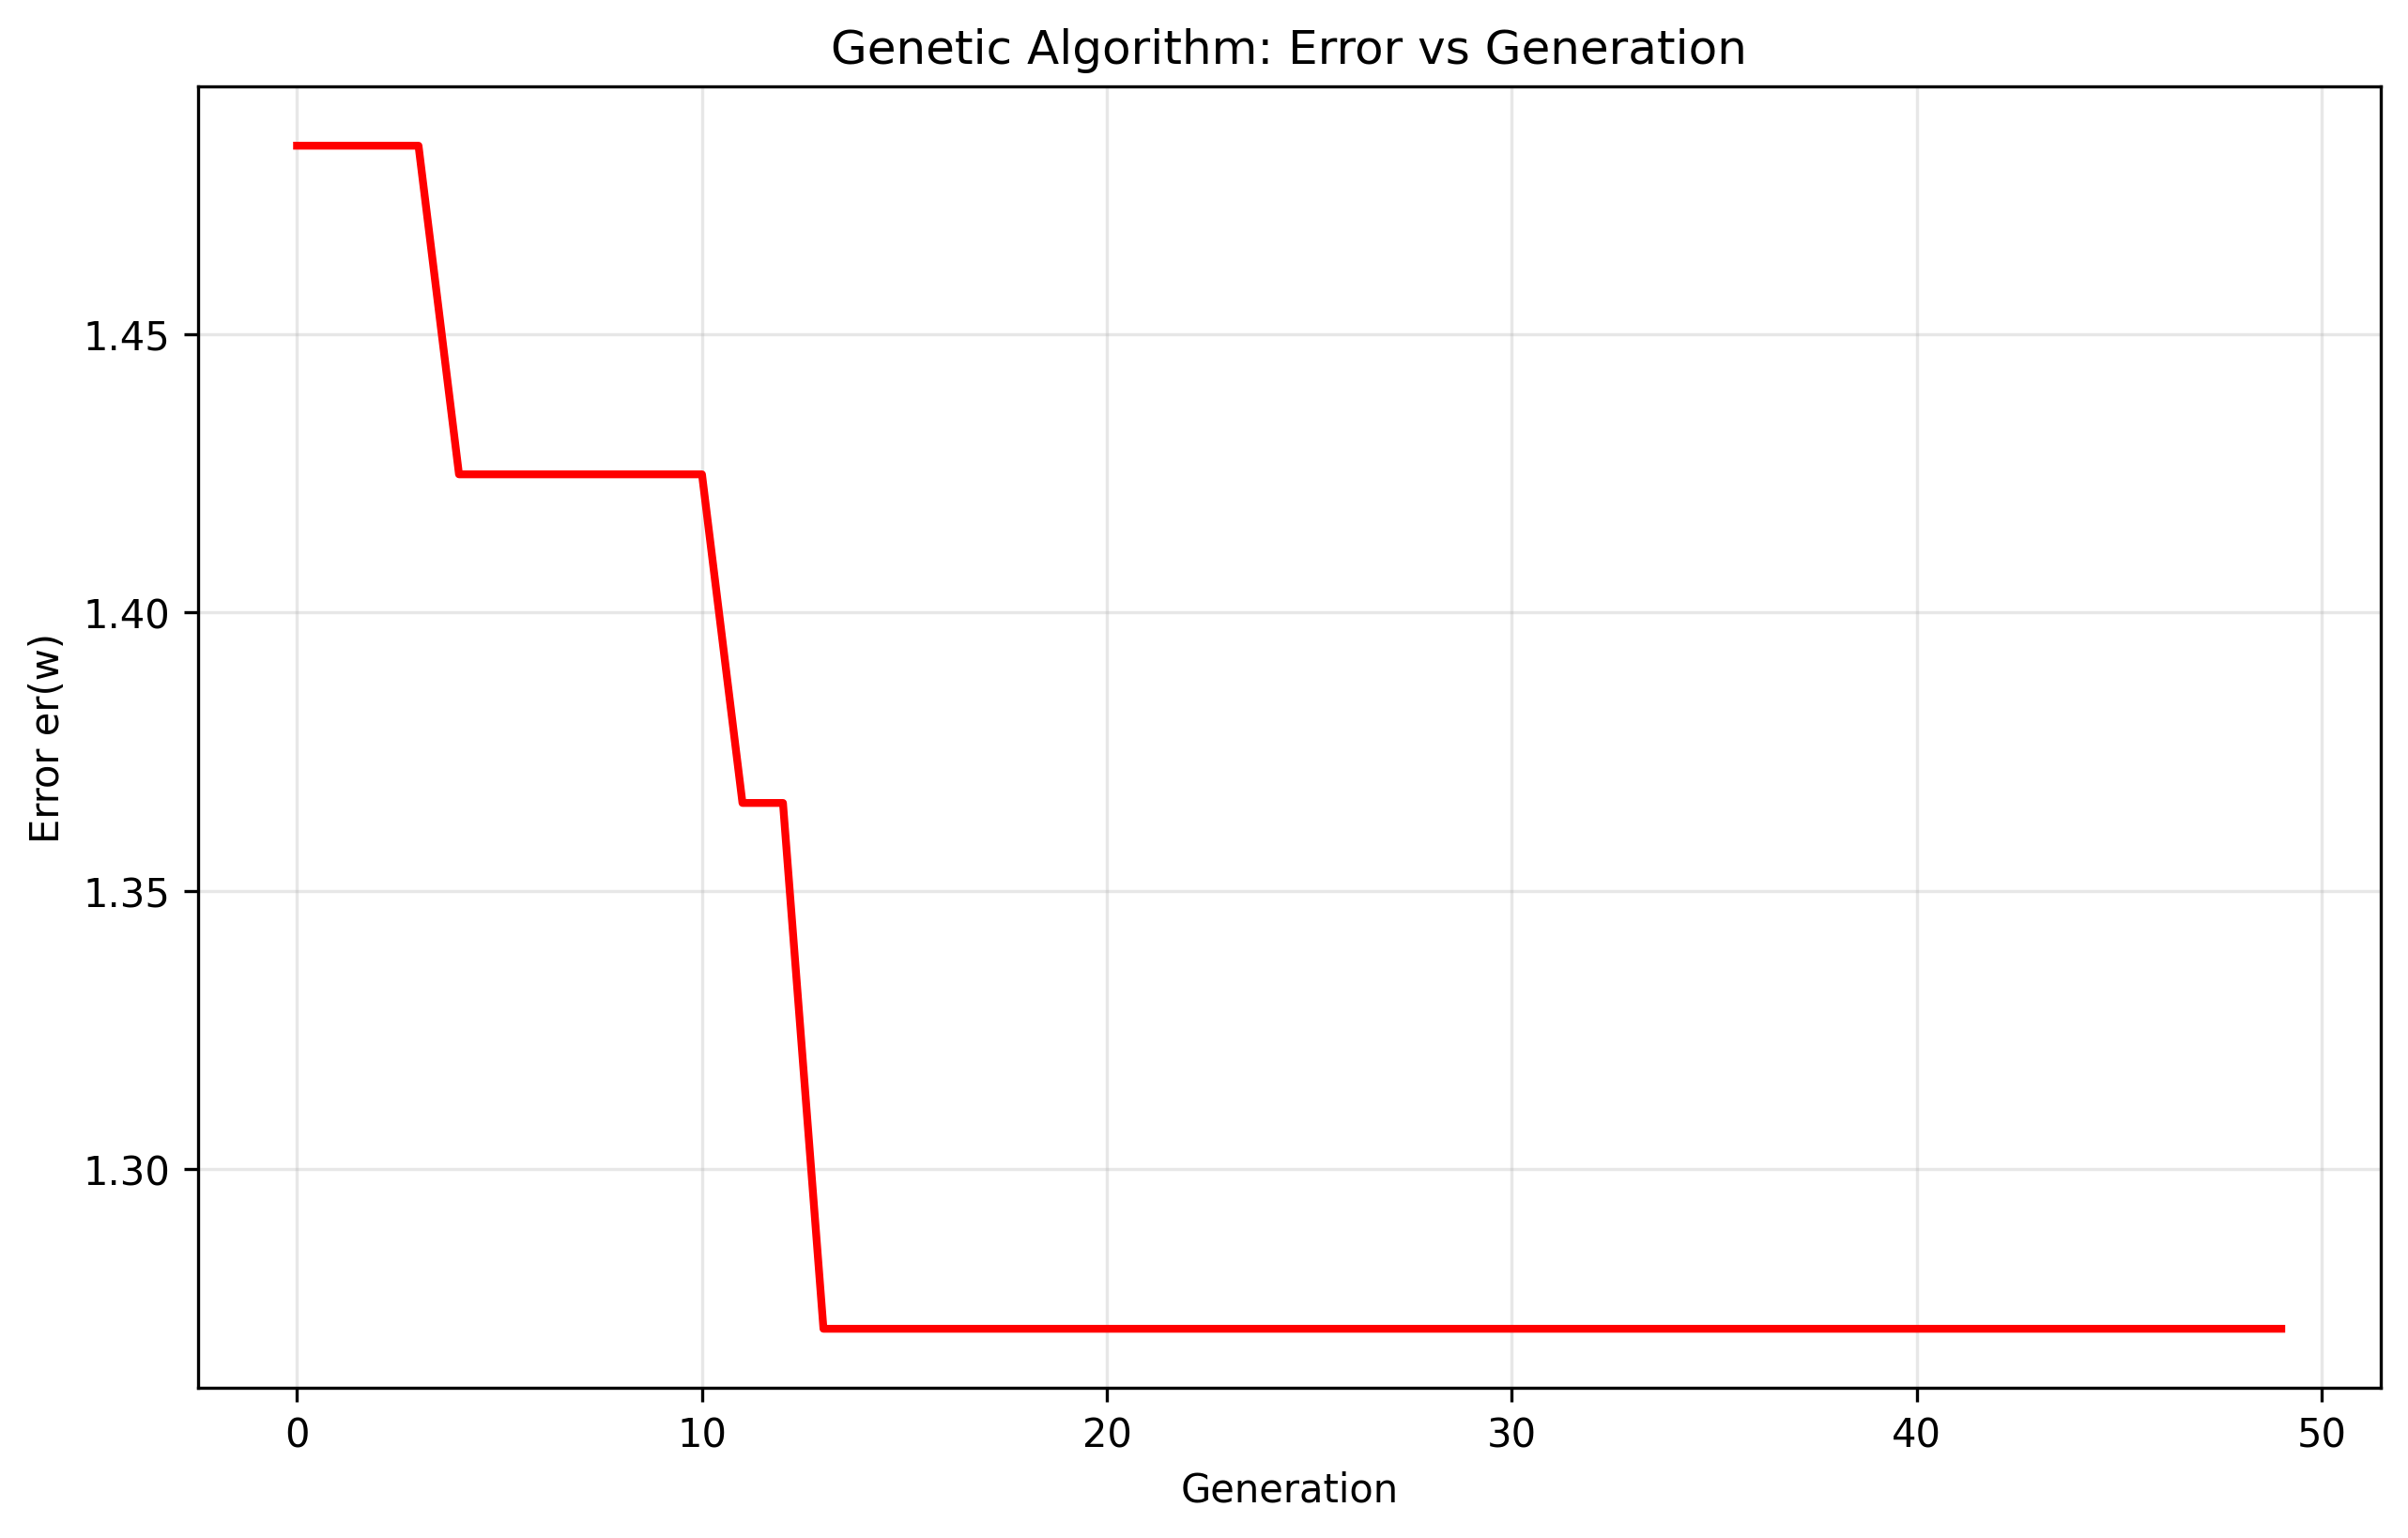
\includegraphics[width=0.75\linewidth]{../../genetic_algorithm_error.png}
    \caption{Error $er(w)$ versus generation for genetic algorithm}
    \label{fig:genetic}
\end{figure}

\subsection*{\textit{(4)} Optimal Solution}

The optimal weight vector $w$ and corresponding error $er(w)$ returned by the genetic algorithm are:

\setcounter{equation}{7}
\begin{equation}
\label{eq:w_genetic}
w = [1, -1, 1, -1, 1, 1]
\end{equation}

\begin{equation}
\label{eq:er_genetic}
er(w) = 1.2713864306784661
\end{equation}

\end{document}

